\section{Ontwerp}
\subsection{Solver}
Als de gebruiker op de knop 'solve' drukt wordt onze solver aangeroepen, deze leest de probleeminstantie in en verwerkt deze. Uiteindelijk geeft de solver weer informatie terug aan de tool, die de informatie weergeeft op het scherm. Deze informatie bestaat onder andere uit de chains en de flexibiliteitsintervallen.

De solver bestaat grofweg uit drie componenten namelijk het ESTA$^+$ algoritme, het chaining algoritme en een algoritme voor het berekenen van de flexibiliteitsintervallen. Het ESTA$^+$ algoritme was al ge\"implementeerd door onze voorgangers en hieraan hebben wij ook niets veranderd. Het chaining algoritme uitgelegt in [??] hebben we zelf ge\"implementeerd. De code voor het berekenen van de flexibiliteitsintervallen bouwt een LP-probleem op en lost deze vervolgens op met COIN LP (Clp). 

\newpage
\begin{figure}[H]
\centering
\label{fig:sd}
\ifx\du\undefined
  \newlength{\du}
\fi
\setlength{\du}{15\unitlength}
\begin{sideways}
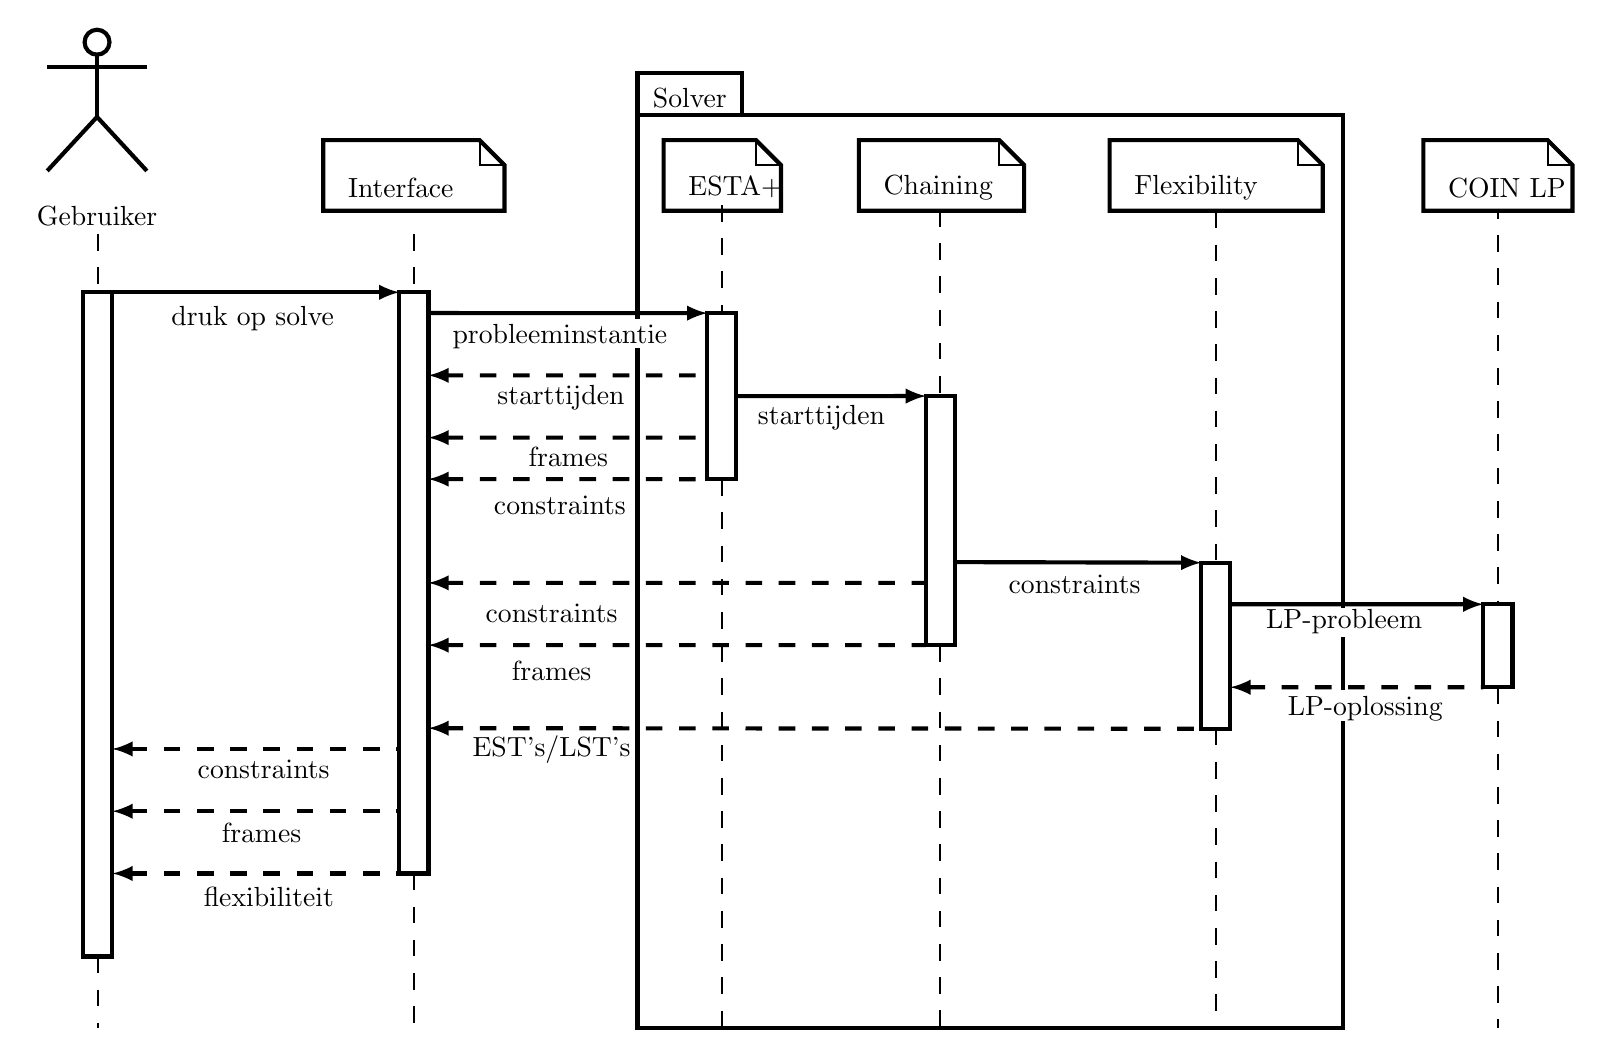
\begin{tikzpicture}
\pgftransformxscale{1.000000}
\pgftransformyscale{-1.000000}
\definecolor{dialinecolor}{rgb}{0.000000, 0.000000, 0.000000}
\pgfsetstrokecolor{dialinecolor}
\definecolor{dialinecolor}{rgb}{1.000000, 1.000000, 1.000000}
\pgfsetfillcolor{dialinecolor}
\pgfsetlinewidth{0.100000\du}
\pgfsetdash{}{0pt}
\definecolor{dialinecolor}{rgb}{1.000000, 1.000000, 1.000000}
\pgfsetfillcolor{dialinecolor}
\fill (29.069200\du,8.000000\du)--(29.069200\du,30.000000\du)--(46.069200\du,30.000000\du)--(46.069200\du,8.000000\du)--cycle;
\definecolor{dialinecolor}{rgb}{0.000000, 0.000000, 0.000000}
\pgfsetstrokecolor{dialinecolor}
\draw (29.069200\du,8.000000\du)--(29.069200\du,30.000000\du)--(46.069200\du,30.000000\du)--(46.069200\du,8.000000\du)--cycle;
\definecolor{dialinecolor}{rgb}{1.000000, 1.000000, 1.000000}
\pgfsetfillcolor{dialinecolor}
\fill (29.069200\du,7.000000\du)--(29.069200\du,8.000000\du)--(31.579200\du,8.000000\du)--(31.579200\du,7.000000\du)--cycle;
\definecolor{dialinecolor}{rgb}{0.000000, 0.000000, 0.000000}
\pgfsetstrokecolor{dialinecolor}
\draw (29.069200\du,7.000000\du)--(29.069200\du,8.000000\du)--(31.579200\du,8.000000\du)--(31.579200\du,7.000000\du)--cycle;
% setfont left to latex
\definecolor{dialinecolor}{rgb}{0.000000, 0.000000, 0.000000}
\pgfsetstrokecolor{dialinecolor}
\node[anchor=west] at (29.169200\du,7.600000\du){Solver};
\pgfsetlinewidth{0.000000\du}
\pgfsetdash{}{0pt}
\pgfsetdash{}{0pt}
\pgfsetmiterjoin
\definecolor{dialinecolor}{rgb}{1.000000, 1.000000, 1.000000}
\pgfsetfillcolor{dialinecolor}
\fill (45.984921\du,21.864133\du)--(45.984921\du,22.599904\du)--(46.126761\du,22.599904\du)--(46.126761\du,21.864133\du)--cycle;
\definecolor{dialinecolor}{rgb}{1.000000, 1.000000, 1.000000}
\pgfsetstrokecolor{dialinecolor}
\draw (45.984921\du,21.864133\du)--(45.984921\du,22.599904\du)--(46.126761\du,22.599904\du)--(46.126761\du,21.864133\du)--cycle;
\pgfsetlinewidth{0.000000\du}
\pgfsetdash{}{0pt}
\pgfsetdash{}{0pt}
\pgfsetmiterjoin
\definecolor{dialinecolor}{rgb}{1.000000, 1.000000, 1.000000}
\pgfsetfillcolor{dialinecolor}
\fill (46.000640\du,19.882377\du)--(46.000640\du,20.567260\du)--(46.142480\du,20.567260\du)--(46.142480\du,19.882377\du)--cycle;
\definecolor{dialinecolor}{rgb}{1.000000, 1.000000, 1.000000}
\pgfsetstrokecolor{dialinecolor}
\draw (46.000640\du,19.882377\du)--(46.000640\du,20.567260\du)--(46.142480\du,20.567260\du)--(46.142480\du,19.882377\du)--cycle;
\pgfsetlinewidth{0.000000\du}
\pgfsetdash{}{0pt}
\pgfsetdash{}{0pt}
\pgfsetmiterjoin
\definecolor{dialinecolor}{rgb}{1.000000, 1.000000, 1.000000}
\pgfsetfillcolor{dialinecolor}
\fill (28.994166\du,12.926291\du)--(28.994166\du,13.611175\du)--(29.136006\du,13.611175\du)--(29.136006\du,12.926291\du)--cycle;
\definecolor{dialinecolor}{rgb}{1.000000, 1.000000, 1.000000}
\pgfsetstrokecolor{dialinecolor}
\draw (28.994166\du,12.926291\du)--(28.994166\du,13.611175\du)--(29.136006\du,13.611175\du)--(29.136006\du,12.926291\du)--cycle;
\pgfsetlinewidth{0.050000\du}
\pgfsetdash{}{0pt}
\pgfsetdash{{0.400000\du}{0.400000\du}}{0\du}
\definecolor{dialinecolor}{rgb}{0.000000, 0.000000, 0.000000}
\pgfsetstrokecolor{dialinecolor}
\draw (23.683300\du,10.875000\du)--(23.683300\du,12.275000\du);
\definecolor{dialinecolor}{rgb}{0.000000, 0.000000, 0.000000}
\pgfsetstrokecolor{dialinecolor}
\draw (23.683300\du,26.275000\du)--(23.683300\du,29.983241\du);
\pgfsetlinewidth{0.100000\du}
\pgfsetdash{}{0pt}
\definecolor{dialinecolor}{rgb}{1.000000, 1.000000, 1.000000}
\pgfsetfillcolor{dialinecolor}
\fill (23.333300\du,12.275000\du)--(23.333300\du,26.275000\du)--(24.033300\du,26.275000\du)--(24.033300\du,12.275000\du)--cycle;
\definecolor{dialinecolor}{rgb}{0.000000, 0.000000, 0.000000}
\pgfsetstrokecolor{dialinecolor}
\draw (23.333300\du,12.275000\du)--(23.333300\du,26.275000\du)--(24.033300\du,26.275000\du)--(24.033300\du,12.275000\du)--cycle;
\pgfsetlinewidth{0.100000\du}
\pgfsetdash{}{0pt}
\definecolor{dialinecolor}{rgb}{1.000000, 1.000000, 1.000000}
\pgfsetfillcolor{dialinecolor}
\pgfpathellipse{\pgfpoint{16.050000\du}{6.250000\du}}{\pgfpoint{0.300000\du}{0\du}}{\pgfpoint{0\du}{0.300000\du}}
\pgfusepath{fill}
\definecolor{dialinecolor}{rgb}{0.000000, 0.000000, 0.000000}
\pgfsetstrokecolor{dialinecolor}
\pgfpathellipse{\pgfpoint{16.050000\du}{6.250000\du}}{\pgfpoint{0.300000\du}{0\du}}{\pgfpoint{0\du}{0.300000\du}}
\pgfusepath{stroke}
\definecolor{dialinecolor}{rgb}{0.000000, 0.000000, 0.000000}
\pgfsetstrokecolor{dialinecolor}
\draw (14.850000\du,6.850000\du)--(17.250000\du,6.850000\du);
\definecolor{dialinecolor}{rgb}{0.000000, 0.000000, 0.000000}
\pgfsetstrokecolor{dialinecolor}
\draw (16.050000\du,6.550000\du)--(16.050000\du,8.050000\du);
\definecolor{dialinecolor}{rgb}{0.000000, 0.000000, 0.000000}
\pgfsetstrokecolor{dialinecolor}
\draw (16.050000\du,8.050000\du)--(14.850000\du,9.350000\du);
\definecolor{dialinecolor}{rgb}{0.000000, 0.000000, 0.000000}
\pgfsetstrokecolor{dialinecolor}
\draw (16.050000\du,8.050000\du)--(17.250000\du,9.350000\du);
% setfont left to latex
\definecolor{dialinecolor}{rgb}{0.000000, 0.000000, 0.000000}
\pgfsetstrokecolor{dialinecolor}
\node at (16.050000\du,10.445000\du){Gebruiker};
\pgfsetlinewidth{0.100000\du}
\pgfsetdash{}{0pt}
\definecolor{dialinecolor}{rgb}{1.000000, 1.000000, 1.000000}
\pgfsetfillcolor{dialinecolor}
\fill (21.500000\du,8.609620\du)--(25.265000\du,8.609620\du)--(25.865000\du,9.209620\du)--(25.865000\du,10.309620\du)--(21.500000\du,10.309620\du)--cycle;
\definecolor{dialinecolor}{rgb}{0.000000, 0.000000, 0.000000}
\pgfsetstrokecolor{dialinecolor}
\draw (21.500000\du,8.609620\du)--(25.265000\du,8.609620\du)--(25.865000\du,9.209620\du)--(25.865000\du,10.309620\du)--(21.500000\du,10.309620\du)--cycle;
\pgfsetlinewidth{0.050000\du}
\definecolor{dialinecolor}{rgb}{0.000000, 0.000000, 0.000000}
\pgfsetstrokecolor{dialinecolor}
\draw (25.265000\du,8.609620\du)--(25.265000\du,9.209620\du)--(25.865000\du,9.209620\du);
% setfont left to latex
\definecolor{dialinecolor}{rgb}{0.000000, 0.000000, 0.000000}
\pgfsetstrokecolor{dialinecolor}
\node[anchor=west] at (21.850000\du,9.754620\du){Interface};
\pgfsetlinewidth{0.100000\du}
\pgfsetdash{}{0pt}
\definecolor{dialinecolor}{rgb}{1.000000, 1.000000, 1.000000}
\pgfsetfillcolor{dialinecolor}
\fill (29.700000\du,8.609620\du)--(31.925000\du,8.609620\du)--(32.525000\du,9.209620\du)--(32.525000\du,10.309620\du)--(29.700000\du,10.309620\du)--cycle;
\definecolor{dialinecolor}{rgb}{0.000000, 0.000000, 0.000000}
\pgfsetstrokecolor{dialinecolor}
\draw (29.700000\du,8.609620\du)--(31.925000\du,8.609620\du)--(32.525000\du,9.209620\du)--(32.525000\du,10.309620\du)--(29.700000\du,10.309620\du)--cycle;
\pgfsetlinewidth{0.050000\du}
\definecolor{dialinecolor}{rgb}{0.000000, 0.000000, 0.000000}
\pgfsetstrokecolor{dialinecolor}
\draw (31.925000\du,8.609620\du)--(31.925000\du,9.209620\du)--(32.525000\du,9.209620\du);
% setfont left to latex
\definecolor{dialinecolor}{rgb}{0.000000, 0.000000, 0.000000}
\pgfsetstrokecolor{dialinecolor}
\node[anchor=west] at (30.050000\du,9.754620\du){ESTA+};
\pgfsetlinewidth{0.050000\du}
\pgfsetdash{}{0pt}
\pgfsetdash{{0.400000\du}{0.400000\du}}{0\du}
\definecolor{dialinecolor}{rgb}{0.000000, 0.000000, 0.000000}
\pgfsetstrokecolor{dialinecolor}
\draw (16.070000\du,10.875000\du)--(16.070000\du,12.275000\du);
\definecolor{dialinecolor}{rgb}{0.000000, 0.000000, 0.000000}
\pgfsetstrokecolor{dialinecolor}
\draw (16.070000\du,28.275000\du)--(16.070000\du,30.000000\du);
\pgfsetlinewidth{0.100000\du}
\pgfsetdash{}{0pt}
\definecolor{dialinecolor}{rgb}{1.000000, 1.000000, 1.000000}
\pgfsetfillcolor{dialinecolor}
\fill (15.720000\du,12.275000\du)--(15.720000\du,28.275000\du)--(16.420000\du,28.275000\du)--(16.420000\du,12.275000\du)--cycle;
\definecolor{dialinecolor}{rgb}{0.000000, 0.000000, 0.000000}
\pgfsetstrokecolor{dialinecolor}
\draw (15.720000\du,12.275000\du)--(15.720000\du,28.275000\du)--(16.420000\du,28.275000\du)--(16.420000\du,12.275000\du)--cycle;
\pgfsetlinewidth{0.050000\du}
\pgfsetdash{}{0pt}
\pgfsetdash{{0.400000\du}{0.400000\du}}{0\du}
\definecolor{dialinecolor}{rgb}{0.000000, 0.000000, 0.000000}
\pgfsetstrokecolor{dialinecolor}
\draw (31.100000\du,10.171800\du)--(31.100000\du,12.776672\du);
\definecolor{dialinecolor}{rgb}{0.000000, 0.000000, 0.000000}
\pgfsetstrokecolor{dialinecolor}
\draw (31.100000\du,16.776672\du)--(31.100000\du,30.000000\du);
\pgfsetlinewidth{0.100000\du}
\pgfsetdash{}{0pt}
\definecolor{dialinecolor}{rgb}{1.000000, 1.000000, 1.000000}
\pgfsetfillcolor{dialinecolor}
\fill (30.750000\du,12.776672\du)--(30.750000\du,16.776672\du)--(31.450000\du,16.776672\du)--(31.450000\du,12.776672\du)--cycle;
\definecolor{dialinecolor}{rgb}{0.000000, 0.000000, 0.000000}
\pgfsetstrokecolor{dialinecolor}
\draw (30.750000\du,12.776672\du)--(30.750000\du,16.776672\du)--(31.450000\du,16.776672\du)--(31.450000\du,12.776672\du)--cycle;
\pgfsetlinewidth{0.050000\du}
\pgfsetdash{}{0pt}
\pgfsetdash{{0.400000\du}{0.400000\du}}{0\du}
\definecolor{dialinecolor}{rgb}{0.000000, 0.000000, 0.000000}
\pgfsetstrokecolor{dialinecolor}
\draw (49.797500\du,10.100300\du)--(49.797500\du,19.790678\du);
\definecolor{dialinecolor}{rgb}{0.000000, 0.000000, 0.000000}
\pgfsetstrokecolor{dialinecolor}
\draw (49.797500\du,21.790678\du)--(49.797500\du,30.000000\du);
\pgfsetlinewidth{0.100000\du}
\pgfsetdash{}{0pt}
\definecolor{dialinecolor}{rgb}{1.000000, 1.000000, 1.000000}
\pgfsetfillcolor{dialinecolor}
\fill (49.447500\du,19.790678\du)--(49.447500\du,21.790678\du)--(50.147500\du,21.790678\du)--(50.147500\du,19.790678\du)--cycle;
\definecolor{dialinecolor}{rgb}{0.000000, 0.000000, 0.000000}
\pgfsetstrokecolor{dialinecolor}
\draw (49.447500\du,19.790678\du)--(49.447500\du,21.790678\du)--(50.147500\du,21.790678\du)--(50.147500\du,19.790678\du)--cycle;
\pgfsetlinewidth{0.100000\du}
\pgfsetdash{}{0pt}
\definecolor{dialinecolor}{rgb}{1.000000, 1.000000, 1.000000}
\pgfsetfillcolor{dialinecolor}
\fill (48.000000\du,8.609620\du)--(50.995000\du,8.609620\du)--(51.595000\du,9.209620\du)--(51.595000\du,10.309620\du)--(48.000000\du,10.309620\du)--cycle;
\definecolor{dialinecolor}{rgb}{0.000000, 0.000000, 0.000000}
\pgfsetstrokecolor{dialinecolor}
\draw (48.000000\du,8.609620\du)--(50.995000\du,8.609620\du)--(51.595000\du,9.209620\du)--(51.595000\du,10.309620\du)--(48.000000\du,10.309620\du)--cycle;
\pgfsetlinewidth{0.050000\du}
\definecolor{dialinecolor}{rgb}{0.000000, 0.000000, 0.000000}
\pgfsetstrokecolor{dialinecolor}
\draw (50.995000\du,8.609620\du)--(50.995000\du,9.209620\du)--(51.595000\du,9.209620\du);
% setfont left to latex
\definecolor{dialinecolor}{rgb}{0.000000, 0.000000, 0.000000}
\pgfsetstrokecolor{dialinecolor}
\node[anchor=west] at (48.350000\du,9.754620\du){COIN LP};
\pgfsetlinewidth{0.100000\du}
\pgfsetbuttcap
\pgfsetdash{}{0pt}
{
\definecolor{dialinecolor}{rgb}{0.000000, 0.000000, 0.000000}
\pgfsetfillcolor{dialinecolor}
% was here!!!
\pgfsetarrowsstart{latex}
\definecolor{dialinecolor}{rgb}{0.000000, 0.000000, 0.000000}
\pgfsetstrokecolor{dialinecolor}
\draw (23.333300\du,12.275000\du)--(16.420000\du,12.275000\du);
}
% setfont left to latex
\definecolor{dialinecolor}{rgb}{0.000000, 0.000000, 0.000000}
\pgfsetstrokecolor{dialinecolor}
\node at (19.800000\du,12.900000\du){druk op solve};
\pgfsetlinewidth{0.100000\du}
\pgfsetbuttcap
\pgfsetdash{}{0pt}
{
\definecolor{dialinecolor}{rgb}{0.000000, 0.000000, 0.000000}
\pgfsetfillcolor{dialinecolor}
% was here!!!
\pgfsetarrowsstart{latex}
\definecolor{dialinecolor}{rgb}{0.000000, 0.000000, 0.000000}
\pgfsetstrokecolor{dialinecolor}
\draw (30.750000\du,12.776700\du)--(24.033300\du,12.775000\du);
}
% setfont left to latex
\definecolor{dialinecolor}{rgb}{0.000000, 0.000000, 0.000000}
\pgfsetstrokecolor{dialinecolor}
\node at (27.201700\du,13.350800\du){probleeminstantie};
\pgfsetlinewidth{0.100000\du}
\pgfsetbuttcap
\pgfsetdash{}{0pt}
{
\definecolor{dialinecolor}{rgb}{0.000000, 0.000000, 0.000000}
\pgfsetfillcolor{dialinecolor}
% was here!!!
\pgfsetarrowsstart{latex}
\definecolor{dialinecolor}{rgb}{0.000000, 0.000000, 0.000000}
\pgfsetstrokecolor{dialinecolor}
\draw (49.447500\du,19.790700\du)--(43.350000\du,19.788700\du);
}
% setfont left to latex
\definecolor{dialinecolor}{rgb}{0.000000, 0.000000, 0.000000}
\pgfsetstrokecolor{dialinecolor}
\node at (46.095400\du,20.214700\du){LP-probleem};
\pgfsetlinewidth{0.100000\du}
\pgfsetbuttcap
\pgfsetdash{}{0pt}
\pgfsetdash{{0.400000\du}{0.400000\du}}{0\du}
{
\definecolor{dialinecolor}{rgb}{0.000000, 0.000000, 0.000000}
\pgfsetfillcolor{dialinecolor}
% was here!!!
\pgfsetarrowsstart{latex}
\definecolor{dialinecolor}{rgb}{0.000000, 0.000000, 0.000000}
\pgfsetstrokecolor{dialinecolor}
\draw (24.033300\du,16.775000\du)--(30.750000\du,16.776700\du);
}
% setfont left to latex
\definecolor{dialinecolor}{rgb}{0.000000, 0.000000, 0.000000}
\pgfsetstrokecolor{dialinecolor}
\node at (27.200000\du,17.400800\du){constraints};
\pgfsetlinewidth{0.100000\du}
\pgfsetbuttcap
\pgfsetdash{{0.400000\du}{0.400000\du}}{0\du}
\pgfsetdash{{0.400000\du}{0.400000\du}}{0\du}
{
\definecolor{dialinecolor}{rgb}{0.000000, 0.000000, 0.000000}
\pgfsetfillcolor{dialinecolor}
% was here!!!
\pgfsetarrowsstart{latex}
\definecolor{dialinecolor}{rgb}{0.000000, 0.000000, 0.000000}
\pgfsetstrokecolor{dialinecolor}
\draw (24.033300\du,14.275000\du)--(30.750000\du,14.276700\du);
}
% setfont left to latex
\definecolor{dialinecolor}{rgb}{0.000000, 0.000000, 0.000000}
\pgfsetstrokecolor{dialinecolor}
\node at (27.225078\du,14.800989\du){starttijden};
\pgfsetlinewidth{0.100000\du}
\pgfsetbuttcap
\pgfsetdash{{0.400000\du}{0.400000\du}}{0\du}
\pgfsetdash{{0.400000\du}{0.400000\du}}{0\du}
{
\definecolor{dialinecolor}{rgb}{0.000000, 0.000000, 0.000000}
\pgfsetfillcolor{dialinecolor}
% was here!!!
\pgfsetarrowsstart{latex}
\definecolor{dialinecolor}{rgb}{0.000000, 0.000000, 0.000000}
\pgfsetstrokecolor{dialinecolor}
\draw (24.033300\du,15.775000\du)--(30.750000\du,15.776700\du);
}
% setfont left to latex
\definecolor{dialinecolor}{rgb}{0.000000, 0.000000, 0.000000}
\pgfsetstrokecolor{dialinecolor}
\node at (27.401700\du,16.250800\du){frames};
\pgfsetlinewidth{0.100000\du}
\pgfsetdash{}{0pt}
\definecolor{dialinecolor}{rgb}{1.000000, 1.000000, 1.000000}
\pgfsetfillcolor{dialinecolor}
\fill (34.403300\du,8.609620\du)--(37.783300\du,8.609620\du)--(38.383300\du,9.209620\du)--(38.383300\du,10.309620\du)--(34.403300\du,10.309620\du)--cycle;
\definecolor{dialinecolor}{rgb}{0.000000, 0.000000, 0.000000}
\pgfsetstrokecolor{dialinecolor}
\draw (34.403300\du,8.609620\du)--(37.783300\du,8.609620\du)--(38.383300\du,9.209620\du)--(38.383300\du,10.309620\du)--(34.403300\du,10.309620\du)--cycle;
\pgfsetlinewidth{0.050000\du}
\definecolor{dialinecolor}{rgb}{0.000000, 0.000000, 0.000000}
\pgfsetstrokecolor{dialinecolor}
\draw (37.783300\du,8.609620\du)--(37.783300\du,9.209620\du)--(38.383300\du,9.209620\du);
% setfont left to latex
\definecolor{dialinecolor}{rgb}{0.000000, 0.000000, 0.000000}
\pgfsetstrokecolor{dialinecolor}
\node[anchor=west] at (34.753300\du,9.754620\du){Chaining};
\pgfsetlinewidth{0.050000\du}
\pgfsetdash{}{0pt}
\pgfsetdash{{0.400000\du}{0.400000\du}}{0\du}
\definecolor{dialinecolor}{rgb}{0.000000, 0.000000, 0.000000}
\pgfsetstrokecolor{dialinecolor}
\draw (36.367000\du,10.290600\du)--(36.367000\du,14.774238\du);
\definecolor{dialinecolor}{rgb}{0.000000, 0.000000, 0.000000}
\pgfsetstrokecolor{dialinecolor}
\draw (36.367000\du,20.774238\du)--(36.367000\du,30.000000\du);
\pgfsetlinewidth{0.100000\du}
\pgfsetdash{}{0pt}
\definecolor{dialinecolor}{rgb}{1.000000, 1.000000, 1.000000}
\pgfsetfillcolor{dialinecolor}
\fill (36.017000\du,14.774238\du)--(36.017000\du,20.774238\du)--(36.717000\du,20.774238\du)--(36.717000\du,14.774238\du)--cycle;
\definecolor{dialinecolor}{rgb}{0.000000, 0.000000, 0.000000}
\pgfsetstrokecolor{dialinecolor}
\draw (36.017000\du,14.774238\du)--(36.017000\du,20.774238\du)--(36.717000\du,20.774238\du)--(36.717000\du,14.774238\du)--cycle;
\pgfsetlinewidth{0.100000\du}
\pgfsetdash{}{0pt}
\definecolor{dialinecolor}{rgb}{1.000000, 1.000000, 1.000000}
\pgfsetfillcolor{dialinecolor}
\fill (40.442900\du,8.609620\du)--(44.977900\du,8.609620\du)--(45.577900\du,9.209620\du)--(45.577900\du,10.309620\du)--(40.442900\du,10.309620\du)--cycle;
\definecolor{dialinecolor}{rgb}{0.000000, 0.000000, 0.000000}
\pgfsetstrokecolor{dialinecolor}
\draw (40.442900\du,8.609620\du)--(44.977900\du,8.609620\du)--(45.577900\du,9.209620\du)--(45.577900\du,10.309620\du)--(40.442900\du,10.309620\du)--cycle;
\pgfsetlinewidth{0.050000\du}
\definecolor{dialinecolor}{rgb}{0.000000, 0.000000, 0.000000}
\pgfsetstrokecolor{dialinecolor}
\draw (44.977900\du,8.609620\du)--(44.977900\du,9.209620\du)--(45.577900\du,9.209620\du);
% setfont left to latex
\definecolor{dialinecolor}{rgb}{0.000000, 0.000000, 0.000000}
\pgfsetstrokecolor{dialinecolor}
\node[anchor=west] at (40.792900\du,9.754620\du){Flexibility};
\pgfsetlinewidth{0.050000\du}
\pgfsetdash{}{0pt}
\pgfsetdash{{0.400000\du}{0.400000\du}}{0\du}
\definecolor{dialinecolor}{rgb}{0.000000, 0.000000, 0.000000}
\pgfsetstrokecolor{dialinecolor}
\draw (43.000000\du,10.328100\du)--(43.000000\du,18.788667\du);
\definecolor{dialinecolor}{rgb}{0.000000, 0.000000, 0.000000}
\pgfsetstrokecolor{dialinecolor}
\draw (43.000000\du,22.788667\du)--(43.000000\du,30.000000\du);
\pgfsetlinewidth{0.100000\du}
\pgfsetdash{}{0pt}
\definecolor{dialinecolor}{rgb}{1.000000, 1.000000, 1.000000}
\pgfsetfillcolor{dialinecolor}
\fill (42.650000\du,18.788667\du)--(42.650000\du,22.788667\du)--(43.350000\du,22.788667\du)--(43.350000\du,18.788667\du)--cycle;
\definecolor{dialinecolor}{rgb}{0.000000, 0.000000, 0.000000}
\pgfsetstrokecolor{dialinecolor}
\draw (42.650000\du,18.788667\du)--(42.650000\du,22.788667\du)--(43.350000\du,22.788667\du)--(43.350000\du,18.788667\du)--cycle;
\pgfsetlinewidth{0.100000\du}
\pgfsetbuttcap
\pgfsetdash{}{0pt}
{
\definecolor{dialinecolor}{rgb}{0.000000, 0.000000, 0.000000}
\pgfsetfillcolor{dialinecolor}
% was here!!!
\pgfsetarrowsstart{latex}
\definecolor{dialinecolor}{rgb}{0.000000, 0.000000, 0.000000}
\pgfsetstrokecolor{dialinecolor}
\draw (36.017000\du,14.774200\du)--(31.450000\du,14.776700\du);
}
% setfont left to latex
\definecolor{dialinecolor}{rgb}{0.000000, 0.000000, 0.000000}
\pgfsetstrokecolor{dialinecolor}
\node at (33.500000\du,15.299400\du){starttijden};
\pgfsetlinewidth{0.100000\du}
\pgfsetbuttcap
\pgfsetdash{}{0pt}
\pgfsetdash{{0.400000\du}{0.400000\du}}{0\du}
{
\definecolor{dialinecolor}{rgb}{0.000000, 0.000000, 0.000000}
\pgfsetfillcolor{dialinecolor}
% was here!!!
\pgfsetarrowsstart{latex}
\definecolor{dialinecolor}{rgb}{0.000000, 0.000000, 0.000000}
\pgfsetstrokecolor{dialinecolor}
\draw (24.033300\du,19.275000\du)--(36.017000\du,19.274200\du);
}
% setfont left to latex
\definecolor{dialinecolor}{rgb}{0.000000, 0.000000, 0.000000}
\pgfsetstrokecolor{dialinecolor}
\node at (27.000000\du,19.998600\du){constraints};
\pgfsetlinewidth{0.100000\du}
\pgfsetbuttcap
\pgfsetdash{{0.400000\du}{0.400000\du}}{0\du}
\pgfsetdash{{0.400000\du}{0.400000\du}}{0\du}
{
\definecolor{dialinecolor}{rgb}{0.000000, 0.000000, 0.000000}
\pgfsetfillcolor{dialinecolor}
% was here!!!
\pgfsetarrowsstart{latex}
\definecolor{dialinecolor}{rgb}{0.000000, 0.000000, 0.000000}
\pgfsetstrokecolor{dialinecolor}
\draw (24.033300\du,20.775000\du)--(36.017000\du,20.774200\du);
}
% setfont left to latex
\definecolor{dialinecolor}{rgb}{0.000000, 0.000000, 0.000000}
\pgfsetstrokecolor{dialinecolor}
\node at (27.000000\du,21.398600\du){frames};
\pgfsetlinewidth{0.100000\du}
\pgfsetbuttcap
\pgfsetdash{}{0pt}
{
\definecolor{dialinecolor}{rgb}{0.000000, 0.000000, 0.000000}
\pgfsetfillcolor{dialinecolor}
% was here!!!
\pgfsetarrowsstart{latex}
\definecolor{dialinecolor}{rgb}{0.000000, 0.000000, 0.000000}
\pgfsetstrokecolor{dialinecolor}
\draw (42.650000\du,18.788700\du)--(36.717000\du,18.774200\du);
}
% setfont left to latex
\definecolor{dialinecolor}{rgb}{0.000000, 0.000000, 0.000000}
\pgfsetstrokecolor{dialinecolor}
\node at (39.600000\du,19.300000\du){constraints};
\pgfsetlinewidth{0.100000\du}
\pgfsetbuttcap
\pgfsetdash{}{0pt}
\pgfsetdash{{0.400000\du}{0.400000\du}}{0\du}
{
\definecolor{dialinecolor}{rgb}{0.000000, 0.000000, 0.000000}
\pgfsetfillcolor{dialinecolor}
% was here!!!
\pgfsetarrowsstart{latex}
\definecolor{dialinecolor}{rgb}{0.000000, 0.000000, 0.000000}
\pgfsetstrokecolor{dialinecolor}
\draw (43.350000\du,21.788700\du)--(49.447500\du,21.790700\du);
}
% setfont left to latex
\definecolor{dialinecolor}{rgb}{0.000000, 0.000000, 0.000000}
\pgfsetstrokecolor{dialinecolor}
\node at (46.600000\du,22.300000\du){LP-oplossing};
\pgfsetlinewidth{0.100000\du}
\pgfsetbuttcap
\pgfsetdash{{0.400000\du}{0.400000\du}}{0\du}
\pgfsetdash{{0.400000\du}{0.400000\du}}{0\du}
{
\definecolor{dialinecolor}{rgb}{0.000000, 0.000000, 0.000000}
\pgfsetfillcolor{dialinecolor}
% was here!!!
\pgfsetarrowsstart{latex}
\definecolor{dialinecolor}{rgb}{0.000000, 0.000000, 0.000000}
\pgfsetstrokecolor{dialinecolor}
\draw (24.033300\du,22.775000\du)--(42.650000\du,22.788700\du);
}
% setfont left to latex
\definecolor{dialinecolor}{rgb}{0.000000, 0.000000, 0.000000}
\pgfsetstrokecolor{dialinecolor}
\node at (27.000000\du,23.300000\du){EST's/LST's};
\pgfsetlinewidth{0.100000\du}
\pgfsetbuttcap
\pgfsetdash{{0.400000\du}{0.400000\du}}{0\du}
\pgfsetdash{{0.400000\du}{0.400000\du}}{0\du}
{
\definecolor{dialinecolor}{rgb}{0.000000, 0.000000, 0.000000}
\pgfsetfillcolor{dialinecolor}
% was here!!!
\pgfsetarrowsstart{latex}
\definecolor{dialinecolor}{rgb}{0.000000, 0.000000, 0.000000}
\pgfsetstrokecolor{dialinecolor}
\draw (16.420000\du,23.275000\du)--(23.333300\du,23.275000\du);
}
% setfont left to latex
\definecolor{dialinecolor}{rgb}{0.000000, 0.000000, 0.000000}
\pgfsetstrokecolor{dialinecolor}
\node at (20.063270\du,23.759337\du){constraints};
\pgfsetlinewidth{0.100000\du}
\pgfsetbuttcap
\pgfsetdash{{0.400000\du}{0.400000\du}}{0\du}
\pgfsetdash{{0.400000\du}{0.400000\du}}{0\du}
{
\definecolor{dialinecolor}{rgb}{0.000000, 0.000000, 0.000000}
\pgfsetfillcolor{dialinecolor}
% was here!!!
\pgfsetarrowsstart{latex}
\definecolor{dialinecolor}{rgb}{0.000000, 0.000000, 0.000000}
\pgfsetstrokecolor{dialinecolor}
\draw (16.420000\du,24.775000\du)--(23.333300\du,24.775000\du);
}
% setfont left to latex
\definecolor{dialinecolor}{rgb}{0.000000, 0.000000, 0.000000}
\pgfsetstrokecolor{dialinecolor}
\node at (20.013270\du,25.296832\du){frames};
\pgfsetlinewidth{0.100000\du}
\pgfsetbuttcap
\pgfsetdash{{0.400000\du}{0.400000\du}}{0\du}
\pgfsetdash{{0.400000\du}{0.400000\du}}{0\du}
{
\definecolor{dialinecolor}{rgb}{0.000000, 0.000000, 0.000000}
\pgfsetfillcolor{dialinecolor}
% was here!!!
\pgfsetarrowsstart{latex}
\definecolor{dialinecolor}{rgb}{0.000000, 0.000000, 0.000000}
\pgfsetstrokecolor{dialinecolor}
\draw (16.420000\du,26.275000\du)--(23.333300\du,26.275000\du);
}
% setfont left to latex
\definecolor{dialinecolor}{rgb}{0.000000, 0.000000, 0.000000}
\pgfsetstrokecolor{dialinecolor}
\node at (20.188269\du,26.846825\du){flexibiliteit};
\end{tikzpicture}
\end{sideways}

\caption{Sequencediagram} 
\end{figure}

\newpage
\subsection{Communicatie}
In bestaande versie van de NedTrain Planner bestond er al een communicatieprotocol voor communicatie tussen de NedTrain Planner en de bestaande solver. Deze communicatieregels worden ook gebruikt door de nieuwe solver. 
\begin{itemize}
    \item \texttt{PROGRESS}: geeft een indicatie (in procenten) van de voortgang van het solveproces. De syntax is \texttt{\textquoteleft PROGRESS: <percentage>\textquoteright}.
    \item \texttt{ERROR}: geeft bericht van een interne fout in de solver (een invariant tijdens het solve proces blijkt niet waar te zijn). Dit zou niet mogen optreden.
    \item Een bericht of de instantie succesvol is opgelost. Dit is een regel \texttt{\textquoteleft Instance solved.\textquoteright} of \texttt{\textquoteleft Instance not solved.\textquoteright}.
    \item \texttt{PC}: duidt aan dat een precedence constraint gepost wordt. De syntax is als volgt: \texttt{\textquoteleft PC: <i1> <j1> <i2> <j2>\textquoteright}, waarbij \texttt{<i1> <j1>} de voorgaangde taak aanduidt, en \texttt{<i2> <j2>} de opvolgende taak.
    \item \texttt{STATE}: Geeft een beschrijving van de huidige verzameling groepen (partitie in groepen van de taken) in de solver en de huidige EST en LST van elke groep. De syntax is \texttt{\textquoteleft STATE: <groepen> -1\textquoteright}, waarbij \texttt{-1} als scheidingsteken wordt gebruikt. Het \texttt{<groepen>} blok bevat de specificaties van groepen. Specificatie per groep begint met \texttt{<treinID> <EST> <LST> <\#taken>}. Daarna volgen \texttt{\#taken} taken, aangeduid met \texttt{<projectID>} \\ \texttt{<taakID>}.
    \item \texttt{PEAK}: Deze regel wordt geprint als het solven niet gelukt is, omdat er aan het einde een contention peak was die niet geresolved kon worden. Het formaat is \texttt{\textquoteleft PEAK:\textquoteright \ <time> <resource> <capacity> <lijst taken en groepen> \textquoteleft -1\textquoteright}. Eerst wordt aangegeven waar de peak zich bevindt en de capaciteit. Elke taak of groep wordt gerepresenteerd met \texttt{<treinID> <taakID>}. Voor groepen geldt dat een van de taken die in de groep zitten wordt gegeven als representant. Vanuit de laatste \texttt{STATE} kan worden afgeleid welke groep bedoeld wordt. Deze peak kan door het planprogramma worden gevisualiseerd.
    \item \texttt{MUTEX}: Deze regel wordt geprint als het solven niet gelukt is, omdat er niet kon worden voldaan aan de eis dat wederzijdse uitsluiting moet gelden. Het formaat is hetzelfde als bij \texttt{PEAK}.
\end{itemize}
De nieuwe communicatieregels zijn nodig om de NedTrain Solver te laten communiceren met de nieuwe solver.
\begin{itemize}
    \item \texttt{CHAIN}: De syntax is \texttt{\textquoteleft <resourceID> <chainID> <\#activiteiten> <activiteiten> -1\textquoteright}. Waarbij \texttt{<activiteiten>} een lijst is van \texttt{\#activiteiten} activiteiten met elke activiteit in de vorm \texttt{<projectID> <taakID>}.
    \item \texttt{CLEARSOFTPREC}: De syntax is \texttt{\textquoteleft CLEARSOFTPREC\textquoteright}.
    \item \texttt{FLEX}: Geeft een lijst van EST's en LST's waarmee de flexibiliteitsintervallen bepaald kunnen worden. De syntax is \texttt{\textquoteleft FLEX: <minflex> <flextotaal> <variabelen> -1\textquoteright}. Waarbij \texttt{-1} het einde van de lijst aangeeft en waarbij \texttt{<variabelen>} een lijst is van EST's en LST's met de syntax \texttt{\textquoteleft <projectID> <taakID> - <tijd>\textquoteright} voor de EST en \texttt{\textquoteleft <projectID> <taakID> + <tijd>\textquoteright} voor de LST.
\end{itemize}
